
\documentclass[degree=bachelor,pifootnote]{thuthesis}
\usepackage{thuthesis}
\usepackage{booktabs}
\usepackage{graphicx}
\usepackage{threeparttable}
\usepackage{geometry}
\usepackage{float}
\usepackage{lscape}
\begin{document}
% 封面 
\frontmatter
\thusetup{
    ctitle={关于比特币期权的实证研究},
    cdegree={经济学学士},
    cdepartment={经济管理学院},
    cmajor={经济与金融},
    cauthor={代港凡},
    csupervisor={王茵田}    
}
\begin{cabstract}
    本文利用LedgerX等比特币期权交易所的公开数据,对比特币期权的特性进行了研究。主要分为以下三个步骤:利用经典的Black-Scholes模型对比特币期权进行定价,并得到模型价格与真实价格之间差异;选取比特币交易量、收益率、峰度、非流动性指标等市场因素与期权价值程度、持仓量、到期时间、隐含波动率等自身特性构建回归模型对价格差异进行解释;利用模型价格和真实价格之间的差异构建套利策略,考察比特币市场的有效性以及Black-Scholes模型蕴含的信息价值。本文主要得到了Black-Scholes模型对大量比特币期权的定价结果,同时发现比特币的流动性、期权的时间、隐含波动率溢价等信息对期权的价格差异均有系统性影响,并从期权供需、套利的可能角度做出了解释。同时也发现对于本文用到的套利策略,认购期权相比认沽期权有更稳定的套利收益。
\end{cabstract}
\ckeywords{比特币, 期权, 套利}
\begin{eabstract}
    This research makes use of open data from LedgerX, a bitcoin option exchange, to take a research on some characteristics of bitcoin options. There are mainly three parts in this paper: first I use famous Black-Scholes model to price the options, and get a suitable definition of the difference between real trading price and model(theoretical) price; second I build regression model to explain the difference using some variables: market variables like bitcoin returns, kurtosis, etc., as well as option variables like implied volatility, time to maturity, etc.; third I develop an arbitrage strategy between market price and model price. This research gets pricing results for options in a long time range, and identifies some systematic relationship between pricing difference and variables like bitcoin liquidity, implied volatility premium, etc.. As for the arbitrage strategy developed in this research, call options gains more stable and significant returns compared with puts.
\end{eabstract}
\ekeywords{bitcoin, option, arbitrage}
\makecover
\tableofcontents
\mainmatter
%引言
\chapter{引言}
\section{研究背景}
\par{2008年,中本聪在互联网上发布论文《比特币:一种点对点的现金系统》\cite{Nakamoto_bitcoin:a},随后于2009年成功制造出比特币的第一个区块。比特币是一种建立在区块链技术上的去中心化交易凭证。不同于其他货币依赖中心结算制度,比特币通过分布式账本对每一次交易进行验证。
由于其安全、去中心化的特点,比特币很快吸引了众多投资者,逐渐成为一种重要的金融资产。
目前在世界范围内有数百家比特币交易所,合计交易额接近百亿美元。
}
\par{随着比特币交易市场的成熟,除了直接购买比特币以获得增值的需求之外,投资者对于交易过程中更多样的投机方式(如做空或者波动率交易)、更稳定的风险控制(如套期保值)有了更高的需求。
因此比特币衍生品应运而生。2013年6月,国内第一家比特币期货交易所——796交易所出现。在国际市场上,芝加哥商品交易所(CME)和芝加哥期权交易所(CBOE)于2017年底开始交易受到监管的比特币期货合约。
}
\par{期货合约的收益与未来资产价格完全线性相关,其对冲风险和杠杆交易能力都不能完全满足投资者的需求。随着近年来比特市场的价格和波动都大幅提升,不少交易所尝试将证券市场的期权、互换等衍生品在比特币市场上实现。
其中Deribit(https://www.deribit.com)和LedgerX(https://www.ledgerx.com)为两个交易相对活跃的期权交易所。}
\section{研究成果及意义}
\subsection{研究成果}
期权允许购买者在指定到期日及其之前选择是否以指定价格购买标的资产,是一种非常重要的金融衍生品。
投资者可以利用期权的保护特性进行套期保值,也可以利用其杠杆特性进行投机交易。期权的出现为比特币市场的投资提供了更多样化的选择。
\par{本文针对LedgerX交易所公开的期权交易数据对比特币市场上的期权进行分析。主要得到了以下三个部分的结论:}
\par{第一,通过Black-Scholes模型对市场上的期权进行定价,并得到市场价格与模型价格的偏差,通过基本描述性统计发现,认购期权价格普遍被模型高估,而认沽期权价格普遍被模型低估。时间和价值程度对于价格偏差有明显影响,同时也验证了波动率微笑现象在比特币市场上的存在。}
\par{第二,利用线性回归模型,使用和市场特征、期权特性有关的多个变量解释了期权市场价格和模型价格之间的偏差。期权的波动率溢价、delta值、较低的流动性和比特币市场收益率与交易量对于价格偏差有显著的提升作用,即推动市场价格高于模型估计;而到期时间、看涨期权的价值程度(比特币价格/行权价)则对价格偏差有降低作用。我们从期权市场上的供给和需求、以及期权套利的可行性对这些现象做出了解释。}
\par{第三,以定价模型为基础,按照delta-对冲的思路构建套利组合,在多种套利组合上,认购期权获得了显著为正的收益,而认沽期权并没有。我也尝试结合回归结果对这一现象做出了解释。}
\subsection{研究意义}
\par{这一研究具有如下的意义:}
\par{
  第一,比特币市场以及其期权市场出现时间都较晚,本研究较为及时地利用最新数据进行了分析,证明了经典的Black-Scholes模型具有应用在这类新兴市场金融衍生品的价值。同时实证分析选取了一些具有明确意义的变量,比较全面地探究了影响期权价格的因素。
}
\par{
  第二,本研究对于金融投资具有实践意义。期权是金融市场上重要的套期保值和投机套利工具。本研究构建了相对合理的套利组合,是一种重要的期权投资和对冲手段,为投资者在数字货币市场上的投资提供更多样化的选择。同时,对现有欧式期权的研究也为金融机构在数字货币市场上推出更复杂的衍生品提供了参考。
}
\par{本文接下来几个部分包括:第2章将介绍比特币市场和期权定价领域相关研究;第3章将介绍数据来源并描述数据;第4章将展示定价模型、定价结果以及对定价偏差的解释;第5章将展示对冲策略结果;第6章为结论。}
%文献综述
\chapter{相关研究综述}
\section{期权定价领域研究}
\par{
期权定价问题一直是金融研究中的热点。Black和Scholes提出了经典的Black-Scholes模型\cite{10.2307/1831029},其中包含了一系列关于市场有效性的假设,并且对这一模型在市场上的应用进行了实证检验\cite{J-1972}。他们采用滚动窗口的股价收益波动率方法,对纽交所上部分股票的期权进行定价,同时构建对冲策略,证实利用模型信息买入定价低于市场价格、卖出定价高于市场价格的期权同时卖出和买入对应股票的策略可以获得正向的超额收益。同时通过对不同波动率组别的收益进行分析,发现了对于具有较高波动率的股票,定价模型会高估期权的价格。同时他们也验证了套利策略中包含的交易成本是非常巨大的,可能会阻碍套利的进行。}
\par{
之后有众多研究对Black-Scholes模型进行检验或者作出改进。Chiras和Manaster在1977年的研究中,提出用当日同股票的不同期权的隐含波动率加权得到加权隐含波动率的方法取代历史波动率估计法,并用加权隐含波动率信息为期权定价以及构建对冲组合,获得了显著的超额收益,证明利用B-S模型得到的隐含波动率确实包含有效的信息\cite{CHIRAS1978213}。Macbeth和Merville在1979年的文章中利用多个股票期权对模型进行了全面的实证检验\cite{Jame-1979}。他们采用回归模型得到预测的隐含波动率后进行定价,发现期权的价值程度(当前价格相对行权价格)对模型与真实价格之间的差异有着系统性影响。实值期权的模型预测价格偏高,而虚值期权的模型预测价格偏低,同时差异也随期限的缩短而减小。
}
\par{Black-Scholes模型设定波动率为市场已知且恒定,这一假设未必与事实相符。Heston(1993)将波动率设定为CIR随机模型形式,并得到这一条件下期权价格的解\cite{10.1093/rfs/6.2.327}。而Savickas则通过对Black-Scholes模型、Heston模型和Weibull模型分别构建delta对冲策略,发现随机波动率模型的收益并无显著提升,同时也呈现出明显的波动率微笑现象\cite{Rober-2005}。}
\par{
    Hull和White在2017年的研究则重新利用Black-Scholes模型达到了更好的对冲模型效果,他们考虑了资产价格和波动率的相关性之后,在delta对冲基础之上提出了最优对冲法则\cite{Hull-2017}。其根本思想在于通过对已有对冲误差和delta之间的建模来优化对冲误差。
}
\section{数字货币市场相关研究}
\par{数字货币市场近年来的不断升温也吸引了不少学术界的眼光。在价格发现方面,Makarov等人于2018年发表的文章探究了比特币和其他数字货币市场上的价格形成与效率问题\cite{Makarov-2018}。他们发现在数字货币市场之间存在着规模巨大、时间持续的套利空间,但同时这一空间主要来自于对各国对真实货币跨国流通的管制,而各个国家内部的市场间套利的空间相对较小。这一研究证明了比特币市场的价格发现机制相对仍不完善,为我们套利策略的构建提供了佐证。
}
\section{流动性相关研究}
\par{流动性是影响市场有效性的重要因素之一。Shiller(1984)最早提出了市场上存在着两类投资者——精明投资者和噪声投资者\cite{Rober-1984}。当市场的套利成本为0时,精明投资者能够充分利用市场信息套利,使价格回到有效市场水平;随着套利成本增加,噪声投资者对股价的预期的影响会逐渐增加,导致价格偏离有效市场水平。套利成本涉及交易成本、价格滑点等多种与流动性有关的因素。因此我会加入衡量市场流动性的指标来解释期权真实价格与模型价格之间的差异。我主要选择的指标是Amihud于2002年提出的非流动性指标\cite{Yako-2002}。这一指标通过衡量股价收益率对成交量的敏感性来度量市场的流动性,为目前在全球市场上比较通用的指标,具体公式可见第\ref{research_method}章。}
%数据描述
\chapter{数据}
\section{数据来源}
\subsection{比特币数据}
\par{
    
    本文主要采用期权交易所LedgerX(https://www.ledgerx.com)公开的每日交易数据,数据位于其网站上(data.ledgerx.com),该交易所的所有期权均为欧式期权。数据包括期权合约条款(行权价、是否为认购、到期日)、每日成交量加权平均价、成交量、持仓量、最后一次买价和卖价等。其中一天的数据示例如下图所示:
    \begin{figure}[H]
        \begin{small}
            \begin{center}
                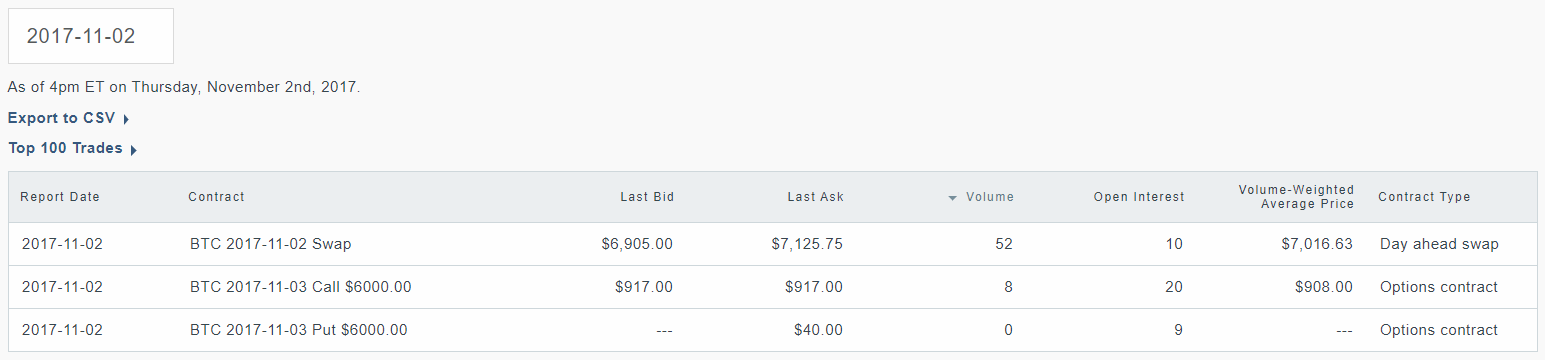
\includegraphics[width=0.95\textwidth]{figures/data_example.png}
            \end{center}
            \caption{LedgerX数据展示}
            \label{data_example}
        \end{small}
    \end{figure}
    利用python爬虫获取了2017年10月17日至2018年12月31日的全部数据,剔除了如图\ref{data_example}中所示的隔夜互换、交易量为0(只有买价或卖价)的数据之后,得到共计1726条期权的交易数据。然而根据参考文献\cite{J-1972}\cite{Jame-1979},一般认为离到期日较近的期权、价值更虚的期权往往定价不准确,因此之后进行回归时会做进一步筛选。
}
\subsection{比特币数据}
\par{
    比特币有众多交易所,根据前述参考文献可知,不同交易所之间价格存在一定差异,且用不同正常货币交易的交易所之间套利空间更为巨大\cite{Makarov-2018},因此这里我们限制选择以美元为交易货币的交易所,根据比特币数据汇总网站Bitcoinity(https://bitcoinity.org)提供数据,可得到所有美元交易所中,每日结算价中最高者和最低者之比,这一比值走势如下图:
    \begin{figure}[H]
        \begin{small}
            \begin{center}
                \includegraphics[width=0.95\textwidth]{figures/maxmin_ratio_plot.png}
            \end{center}
            \caption{交易所间最高价与最低价之比}
            \label{maxmin_ratio}
        \end{small}
    \end{figure}
    }
    \par{从图中可见交易所之间的价格差异在18年初较大,为保证之后回归的准确和套利策略的可行性,我们选择coinmarketcap网站(https://coinmarketcap.com)上公开的各大美元交易所的比特币加权均价,这样可以保证以交易量较大的比特币交易所价格为基础,位于最高者和最低者之间。
    }
\subsection{比特币无风险利率信息}
    \par{各种期权定价模型均需要有无风险利率信息,而比特币市场上并无公开的无风险利率。根据2015年出版的《比特币手册(Bitcoin Handbook)》\cite{WESNER2015223},作者提出了通过宏观经济理论推断比特币无风险利率的方法,根据其提供的结果,可得比特币的无风险利率在4$\%$~6$\%$之间,考虑到利率本身对定价结果影响较小,故取比特币无风险利率为5$\%$。
    }

\section{数据描述}
    \par{
        对数据搜集期比特币每日收盘价数据取对数收益率,按照一年滚动窗口计算其波动率、偏度、峰度。对其描述性统计如下:}

        \begin{threeparttable}[H]
            
            \centering
            \caption{比特币数据描述性统计}
            \label{btc_describe}
            \begin{tabular}{lrrrrr}
\toprule
{} &             成交量 &   对数收益率 &     波动率 &      偏度 &      峰度 \\
\midrule
count &         544.000 & 544.000 & 544.000 & 544.000 & 544.000 \\
mean  &  6749637776.700 &  -0.000 &   0.047 &  -0.096 &   2.667 \\
std   &  3790972106.645 &   0.044 &   0.007 &   0.189 &   0.802 \\
min   &  1403920000.000 &  -0.185 &   0.032 &  -0.541 &   1.656 \\
25\%   &  4273417520.000 &  -0.017 &   0.043 &  -0.313 &   2.135 \\
50\%   &  5470000143.500 &   0.002 &   0.049 &  -0.041 &   2.326 \\
75\%   &  7810741265.500 &   0.018 &   0.054 &   0.060 &   3.032 \\
max   & 23840899072.000 &   0.225 &   0.055 &   0.175 &   5.026 \\
\bottomrule
\end{tabular}

            \begin{tablenotes}
                \footnotesize
                \item 注:波动率、偏度、峰度用一年(365天)滚动窗口估计,均为日化数据;偏度为超额偏度;成交量以美元计量。
            \end{tablenotes}
        \end{threeparttable}
        
    
    ~\\
    \par{
        
        由表\ref{btc_describe}可见,数据期比特币存在一定的负偏度与高峰度。其中峰度一直保持在0以上,说明比特币收益率存在偏峰厚尾现象,而偏度数据相对波动较大,总体上比较接近0偏度,同时对数收益率均值也非常接近0,说明比特币的收益分布非常接近存在尖峰厚尾现象的对称分布。
    }
    \newpage
    \par{
        将期权交易数据按照其标签(即合约的到期日、行权价、认购/认沽方向)分组,并对基本信息统计如下:
    }
    \par{
    \begin{threeparttable}[H]
        \centering
        \caption{期权数据描述性统计}
        \label{option_describe}
        \begin{tabular}{lrrrr}
\toprule
{} &      期限 &       行权价 &  认购期权数量 &  认沽期权数量 \\
\midrule
count & 306.000 &   306.000 & 197.000 & 109.000 \\
mean  &  90.536 &  8867.647 &         &         \\
std   & 141.132 &  6207.192 &         &         \\
min   &   1.000 &  2000.000 &         &         \\
25\%   &   3.250 &  6000.000 &         &         \\
50\%   &  30.000 &  7000.000 &         &         \\
75\%   &  96.750 & 10000.000 &         &         \\
max   & 637.000 & 50000.000 &         &         \\
\bottomrule
\end{tabular}

        \begin{tablenotes}
            \footnotesize
            \item 注:此处统计已将期权按照到期日、行权价和方向分组。期限为第一个有交易的日期至到期日的天数。
        \end{tablenotes}
    \end{threeparttable}
    }
    ~\\
    \par{
    从表\ref{option_describe}可见,认购期权数量略多于认沽期权,行权价的覆盖范围较广。存在一部分期限极短的数据,可能存在之前无交易的情况,会在实证研究中考虑将这类数据删去。
    }
% 研究方法
\chapter{实证研究方法}\label{research_method}
    \section{期权的定价模型}
    本文首先采用Black-Scholes模型对比特币进行定价。Black-Scholes模型对交易资产及其市场有如下假设:
    \begin{itemize}
        \item 存在已知且恒定的无风险收益率r。
        \item 资产价格为带漂移随机游走过程, 即$dS={\mu}Sdt+{\sigma}SdW$,其中价格波动率$\sigma$为已知的常数。可以推导出在这一假设下资产的收益率服从对数正态分布。
        \item 期权为欧式期权,即只有到期时期权的购买者才能够行权。
        \item 买卖期权和标的资产时不会产生交易费用和其他损失。
        \item 能够以无风险利率自由借入借出任意数量的资产。
        \item 对卖空操作无限制。
        \item 不存在无风险套利机会。
        \item 资产不支付红利。
    \end{itemize}
    在以上假设下,可以得到如下的期权定价公式:
    \begin{equation}\label{bs-call}
            C=S*N(d_1)-X*e^{-rT}*N(d_2) 
    \end{equation}
    \begin{equation}\label{bs-put}
        P=X*e^{-rT}*N(-d_2)-S*N(-d_1)
    \end{equation}
    其中
    \begin{equation*}
        \begin{split}
        d_1=\frac{ln(S/X)+(r+\sigma^2/2)T}{\sigma{\sqrt{T}}} \\
        d_2=\frac{ln(S/X)+(r-\sigma^2/2)T}{\sigma{\sqrt{T}}}
        \end{split}
    \end{equation*}
    其中,C为看涨期权价格,P为看跌期权价格,S为标的资产价格,X为行权价格,r为无风险利率,T为距离到期日时间,$\sigma$为资产收益率的波动率。
    
        比起股票或其他传统金融资产,比特币市场一定程度上更符合Black-Scholes模型的假设,也更利于进行推导模型时构建的delta-对冲过程:
        \begin{itemize}
            \item 比特币为连续交易,无假日和休市时间,可以在任意时间买卖。
            \item 比特币可以分割成(足够小的)任意单位买卖,而非必须整数。
        \end{itemize}

    \section{波动率的估计}
    现实中,市场上的真实波动率并非恒定且已知的,因而无法直接采用\ref{bs-call}\ref{bs-put}的公式对期权进行定价。主要可以采用如下几种方式对价格波动率进行估计。
    \subsection{波动率滚动估计}
    投资者在市场上直接观察到的是近期一段时间比特币价格的波动。可以利用滚动窗口得到近期收益率的标准差估计,并将其作为期权到期日期前的期望波动率:
    \begin{equation}\label{volatility-rolling}
        \hat{\sigma}=\sum_{i=1}^{i=N}\frac{(r_{t-i}-\bar{r})^2}{N-1}
    \end{equation}
    其中$\bar{r}$为这一时期的平均收益率。
    \subsection{加权隐含波动率估计}
    从式\ref{bs-call}和\ref{bs-put}可以得出,期权的价格随波动率上升而上升。可以通过现在市场上的均衡期权价格得到一个$\sigma$的解,即为隐含波动率,这一预测方法利用了期权交易中的隐含信息。
    根据参考文献\cite{CHIRAS1978213},每日有多支期权且他们隐含波动率不同时,可以用以下公式获得当日的加权隐含波动率(WISD):
    \begin{equation}
        WISD=\frac{\sum_{j=1}^{N}{ISD_j\frac{\partial{W_j}}{\partial{v_j}}\frac{v_j}{W_j}}}{\sum_{j=1}^{N}{\frac{\partial{W_j}}{\partial{v_j}}\frac{v_j}{W_j}}}
    \end{equation}
    其中 , $WISD$为加权隐含波动率,$ISD_j$为第$j$个期权的隐含波动率,$N$为同一标的资产的期权个数,$\frac{\partial{W_j}}{\partial{v_j}}\frac{v_j}{W_j}$ 为期权价格相对于波动率的弹性。
    
    \section{对定价偏差的解释}
    波动率微笑现象反映出了期权的隐含波动率和其价值程度(即资产价格与行权价之比)存在规律性的关系,同理我们可以探究很多变量对于期权真实价格与模型价格之间偏差的系统性影响。通过构建回归模型并对变量的系数进行分析,我们可以识别不同因素对真实价格偏离部分的影响的方向,并对其做出解释。这些变量主要分为两个方面:比特币市场因素和期权因素。
    \subsection{比特币市场有关变量}
    \begin{itemize}
        \item LR 比特币市场对数收益率
        \item STD 比特币历史波动率
        \item SKEW 比特币历史偏度
        \item AMI Amihud非流动性指标
        \item BTC\_VOL 比特币市场总交易量
        \item MR 当日比特币交易所中价格最高者和最低者之比
    \end{itemize}
    
    这些指标衡量了比特币市场的市场环境。如波动率和偏度反映了投资者所处的风险情况,同时也属于识别出的模型设定问题,而非流动性指标和MR体现了市场的流动性情况,这些都可能造成真实价格同模型价格之间的偏差。
    \subsection{期权自身有关变量}
    \begin{itemize}
        \item DELTA 期权根据Black-Scholes模型计算出的delta
        \item TIME 期权距离到期日的时间
        \item VP 期权的波动率溢价(Volatility Premimum),利用该期权当时的隐含波动率与当天至到期日之间的实现波动率之差计量。
        \item VOL 期权当天交易量                                     
        \item SPR 期权当天公开的买卖价差
        \item OI 期权当天公开的持仓量(open interest)
        \item CALL 哑变量,是否为认购期权,1为认购期权,0为认沽期权。 
    \end{itemize}
    这些指标能够衡量期权自身性质对真实价格的影响,主要是不同性质的期权可能导致投资者对其供给和需求的不平衡会造成期权价格的偏离。
    \section{套利策略}
    B-S模型是基于用股票和无风险债券复制期权而没有套利空间的原理推导出来的。由此可以利用实际价格与模型价格偏离的部分,构建套利策略,这一策略将反映出B-S模型中包含的信息价值。策略详情如下:
    \begin{itemize}
        
    \end{itemize}

%研究结果
\chapter{实证结果}
\section{定价结果}
按照第4章的Black-Scholes模型\ref{bs-call}和\ref{bs-put},对每个期权的每条交易数据,将距离到期期限、数据期的波动率估计(采用滚动估计方式)、利率、当日比特币价格、行权价等信息输入模型,得到Black-Scholes模型定价。期权的真实价格为当天的成交量加权均价。在定价过程中,我们发现部分期权由于深度价外、而且期限较短,几乎没有模型价值,但仍有较高的真实价格,如果用二者数值的绝对差异将无法表现出这种定价差异的真实影响,损失过多的信息,故定义定价偏差为真实价格与模型价格之比即真实价格/模型价格。同时根据参考文献,深度价外期权和期限较短的期权并不适合用B-S模型定价\cite{10.2307/1831029}\cite{Jame-1979}。因此我们对数据做如下清理:
\begin{itemize}
    \item 剔除每日交易量仅有1的记录
    \item 剔除距离到期日在7日之内的记录
    \item 剔除认购期权的相对价值在0.8以下,认沽期权的相对价值在1.25以上的记录
    \item 剔除期权价格不在期权价格合理范围内的记录,这些期权无法按照价格求得隐含波动率。
\end{itemize}
保留共计600条记录。
600条记录的定价偏差的描述性统计以及按认购、认沽期权的分组统计之后结果如下:
~\\
\begin{center}
    \begin{threeparttable}[H]
    
        \begin{small}
            \caption{定价偏差描述统计}
            \label{tab:option_bias_group}
                \begin{tabular}{lrrr}
\toprule
{} &    定价偏差 &  认购期权定价偏差 &  认沽期权定价偏差 \\
\midrule
count & 600.000 &   364.000 &   236.000 \\
mean  &   0.869 &     0.735 &     1.075 \\
std   &   0.526 &     0.289 &     0.711 \\
min   &   0.105 &     0.105 &     0.282 \\
25\%   &   0.614 &     0.537 &     0.739 \\
50\%   &   0.786 &     0.720 &     0.909 \\
75\%   &   0.997 &     0.886 &     1.162 \\
max   &   5.843 &     2.453 &     5.843 \\
\bottomrule
\end{tabular}

                
        \end{small} 
    \end{threeparttable}
\end{center}
可见在合理的相对价值区间内,真实价格和模型价格差异仍然较大,最大接近6倍。最小接近十分之一,平均水平低于1,说明总体真实价格略低于模型价格。分组结果中,认购期权的平均偏差低于1,而认沽期权的平均偏差高于1,说明平均情况下,认购期权通常价格被低估,而认沽期权通常价格被高估。
~\\
为了初步展示定价偏差和期权价值程度之间的关系,我按照期权的相对价值(比特币价格/行权价)和期限分组,统计了各个组内定价偏差的平均值,以下是定价绝对偏差分组统计的结果:
~\\
\begin{center}
    \begin{threeparttable}[H]
        \centering
        \begin{small}
            \caption{定价偏差分组统计}
            \label{tab:option_bias_group}
                \begin{tabular}{lrrrrr}
\toprule
time\_cut &  0, 30 &  30, 60 &  60, 180 &  180, 624 &  mean \\
moneyness\_cut &          &           &            &             &       \\
\midrule
0.0, 0.6    &    1.027 &     1.126 &      1.075 &       1.129 & 1.109 \\
0.6, 0.9    &    0.822 &     0.968 &      0.911 &       1.029 & 0.937 \\
0.9, 1.1    &    0.812 &     0.774 &      0.953 &       1.102 & 0.843 \\
1.1, 3.9    &    1.010 &     1.054 &      1.016 &       1.185 & 1.063 \\
mean          &    0.856 &     0.903 &      0.961 &       1.098 &       \\
\bottomrule
\end{tabular}

                \begin{tablenotes}
                    \footnotesize
                    \item 注:money\_cut指期权价值程度分组边界(比特币价格/行权价),time\_cut指距到期期限分组边界。
                    
                \end{tablenotes}
        \end{small}
    \end{threeparttable}
        
\end{center}
~\\
可以看到,定价偏差随期限的上升呈增长趋势。对认购和认沽期权分别分组统计,结果如下:
~\\
\begin{center}
    \begin{threeparttable}[H]
        \begin{small}
            \caption{定价偏差分组统计:认购期权}
            \label{tab:call_option_bias_group}
                \begin{tabular}{lrrrrr}
\toprule
time\_cut &  0, 30 &  30, 60 &  60, 180 &  180, 624 &  mean \\
moneyness\_cut &          &           &            &             &       \\
\midrule
0.0, 0.6    &          &     1.167 &      1.073 &       1.129 & 1.113 \\
0.6, 0.9    &    0.789 &     0.964 &      0.891 &       1.027 & 0.924 \\
0.9, 1.1    &    0.769 &     0.725 &      0.806 &       0.932 & 0.770 \\
1.1, 3.9    &    0.937 &     1.032 &      0.875 &       0.941 & 0.939 \\
mean          &    0.797 &     0.870 &      0.911 &       1.063 &       \\
\bottomrule
\end{tabular}

        \end{small}
    \end{threeparttable}
        
\end{center}
~\\
认沽期权分组统计结果:
~\\
\begin{center}
    \begin{threeparttable}[H]
        \begin{small}
            \caption{定价偏差分组统计:认沽期权}
            \label{tab:put_option_bias_group}
                \begin{tabular}{lrrrrr}
\toprule
time\_cut &  0, 30 &  30, 60 &  60, 180 &  180, 624 &  mean \\
moneyness\_cut &          &           &            &             &       \\
\midrule
0.0, 0.6    &    1.027 &     1.003 &      1.104 &             & 1.042 \\
0.6, 0.9    &    0.981 &     1.011 &      1.137 &       1.045 & 1.035 \\
0.9, 1.1    &    0.880 &     0.924 &      1.155 &       1.303 & 0.975 \\
1.1, 3.9    &    1.058 &     1.058 &      1.051 &       1.302 & 1.115 \\
mean          &    0.951 &     0.997 &      1.107 &       1.234 &       \\
\bottomrule
\end{tabular}

    
        \end{small}
    \end{threeparttable}
        
\end{center}
~\\
从分组结果直观而言,对认沽期权实值期权的偏差要小于虚值期权,而对于认购期权这一现象并不明显。
\section{隐含波动率}
隐含波动率即使得Black-Scholes模型价格等于真实价格的波动率参数,这一数值表示了隐含于期权市场价格中与波动率有关的信息。以期权相对价值(S/K)将全部期权分为五组,并求各组平均隐含波动率,以各组相对价值中位数为横轴,隐含波动率为纵轴绘制折线图如下:
\begin{figure}[H]
    \begin{small}
        \begin{center}
            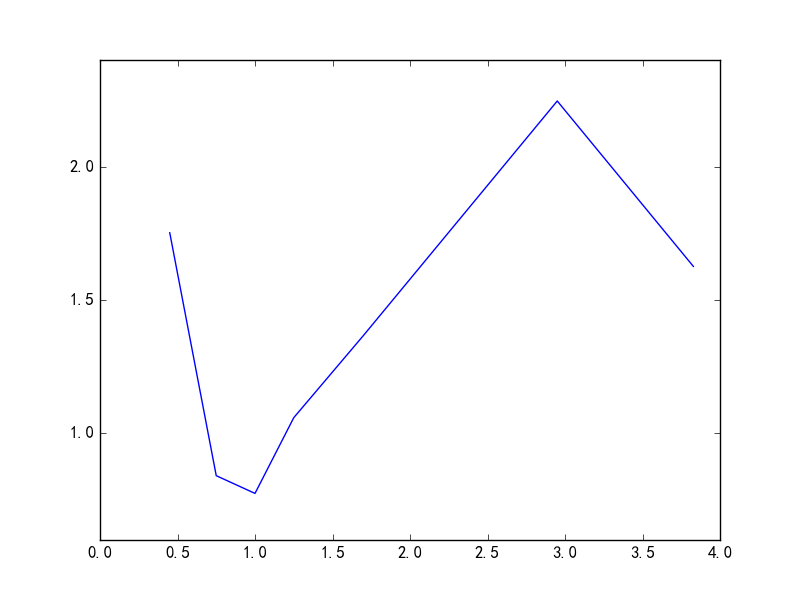
\includegraphics[width=0.95\textwidth]{figures/mean_isd.png}
        \end{center}
        \caption{隐含波动率分组曲线}
        \label{fig:mean_isd}
    \end{small}
\end{figure}
图像呈现出一定的“波动率微笑”性质,相对价值接近1的时候隐含波动率水平更低。本质上隐含波动率微笑现象反映了收益分布与对数正态分布之间的差异。为此我们可以构建两个在回归模型中需要用到的变量。
\par{
    波动率溢价:定义为从现在至期权到期日期间比特币波动率与期权隐含波动率之差。由于波动率越大,一般期权的价格越高,这一指标衡量了期权交易者对波动率的预测与未来期权波动率符合程度。
}

\section{回归模型}
我们首先构建第\ref{reg vars}节提出的变量,并对其进行描述性统计。变量的描述统计和相关性矩阵如下:
\newpage
\newgeometry{top=1cm,bottom=1cm
}
\begin{landscape} 
    \begin{table}[H]
        \caption{解释变量的描述性统计}
        \resizebox{\linewidth}{!}{
        \begin{tabular}{lrrrrrrrrrrrrrrrrr}
\toprule
{} &  log\_ret &  volatility &  skewness &  amihud &  maxmin\_ratio &  btc\_volume &   time &  const\_delta\_5 &  vol\_pre &  spread &  open\_interest &  slope &  volume &  contract\_is\_call &  inter\_call\_money &  inter\_put\_money &  inter\_call\_skewness \\
\midrule
count &   577.00 &      577.00 &    577.00 &  577.00 &        577.00 &      577.00 & 577.00 &         577.00 &   577.00 &  577.00 &         577.00 & 577.00 &  577.00 &            577.00 &            577.00 &           577.00 &               577.00 \\
mean  &    -0.00 &        0.04 &     -0.39 &    0.04 &          1.04 &       22.45 &   3.75 &           0.14 &     0.01 &  272.88 &          62.84 &   0.00 &   19.48 &              0.60 &              0.58 &             0.41 &                -0.24 \\
std   &     0.05 &        0.02 &      0.76 &    0.02 &          0.03 &        0.40 &   1.00 &           0.47 &     0.02 &  430.01 &          99.58 &   0.00 &   29.35 &              0.49 &              0.50 &             0.51 &                 0.61 \\
min   &    -0.17 &        0.01 &     -4.50 &    0.01 &          1.00 &       21.30 &   2.08 &          -1.00 &    -0.06 & -225.00 &           0.00 &  -0.00 &    2.00 &              0.00 &              0.00 &             0.00 &                -4.50 \\
25\%   &    -0.03 &        0.03 &     -0.81 &    0.03 &          1.01 &       22.16 &   3.09 &          -0.31 &    -0.00 &  121.50 &           9.00 &  -0.00 &    3.00 &              0.00 &              0.00 &             0.00 &                -0.40 \\
50\%   &     0.00 &        0.04 &     -0.23 &    0.04 &          1.03 &       22.36 &   3.56 &           0.36 &     0.01 &  174.00 &          31.00 &   0.00 &    7.00 &              1.00 &              0.86 &             0.00 &                -0.00 \\
75\%   &     0.02 &        0.05 &      0.03 &    0.05 &          1.05 &       22.65 &   4.39 &           0.53 &     0.02 &  310.75 &          98.00 &   0.00 &   20.00 &              1.00 &              0.95 &             0.98 &                 0.00 \\
max   &     0.23 &        0.09 &      1.15 &    0.09 &          1.19 &       23.89 &   6.36 &           1.00 &     0.11 & 9000.00 &        1109.00 &   0.00 &  226.00 &              1.00 &              3.83 &             1.25 &                 1.03 \\
\bottomrule
\end{tabular}

        }
    \end{table}
    \begin{table}[H]
        \caption{解释变量的相关性矩阵}
        \resizebox{\linewidth}{!}{\begin{tabular}{lrrrrrrrrrrrrrrrrr}
\toprule
{} &  log\_ret &  volatility &  skewness &  amihud &  maxmin\_ratio &  btc\_volume &  time &  delta\_5 &  vol\_pre &  spread &  open\_interest &  slope &  volume &  contract\_is\_call &  inter\_call\_money &  inter\_put\_money &  inter\_call\_skewness \\
\midrule
log\_ret             &     1.00 &        0.02 &      0.13 &    0.03 &         -0.12 &       -0.01 &  0.05 &     0.09 &    -0.14 &   -0.02 &          -0.01 &   0.06 &   -0.02 &              0.03 &              0.05 &            -0.00 &                 0.08 \\
volatility          &     0.02 &        1.00 &      0.29 &    0.98 &          0.64 &        0.75 &  0.20 &     0.08 &     0.27 &    0.35 &          -0.20 &   0.07 &   -0.14 &             -0.13 &             -0.11 &             0.14 &                 0.23 \\
skewness            &     0.13 &        0.29 &      1.00 &    0.35 &          0.07 &        0.17 &  0.10 &     0.10 &     0.15 &    0.13 &           0.03 &   0.03 &   -0.06 &              0.01 &              0.05 &             0.00 &                 0.80 \\
amihud              &     0.03 &        0.98 &      0.35 &    1.00 &          0.61 &        0.71 &  0.19 &     0.08 &     0.27 &    0.33 &          -0.20 &   0.07 &   -0.15 &             -0.14 &             -0.11 &             0.15 &                 0.29 \\
maxmin\_ratio        &    -0.12 &        0.64 &      0.07 &    0.61 &          1.00 &        0.64 &  0.15 &     0.06 &    -0.02 &    0.35 &          -0.21 &   0.06 &   -0.13 &             -0.10 &             -0.04 &             0.10 &                 0.07 \\
btc\_volume          &    -0.01 &        0.75 &      0.17 &    0.71 &          0.64 &        1.00 &  0.14 &     0.09 &     0.17 &    0.36 &          -0.17 &   0.10 &   -0.10 &             -0.09 &             -0.03 &             0.10 &                 0.14 \\
time                &     0.05 &        0.20 &      0.10 &    0.19 &          0.15 &        0.14 &  1.00 &     0.17 &     0.21 &    0.32 &           0.02 &  -0.08 &   -0.02 &              0.15 &             -0.08 &            -0.12 &                 0.01 \\
delta\_5             &     0.09 &        0.08 &      0.10 &    0.08 &          0.06 &        0.09 &  0.17 &     1.00 &    -0.15 &    0.16 &          -0.00 &  -0.08 &    0.03 &              0.81 &              0.85 &            -0.73 &                -0.13 \\
vol\_pre             &    -0.14 &        0.27 &      0.15 &    0.27 &         -0.02 &        0.17 &  0.21 &    -0.15 &     1.00 &    0.20 &           0.07 &  -0.05 &   -0.02 &             -0.12 &             -0.18 &             0.10 &                 0.13 \\
spread              &    -0.02 &        0.35 &      0.13 &    0.33 &          0.35 &        0.36 &  0.32 &     0.16 &     0.20 &    1.00 &          -0.10 &   0.02 &   -0.08 &              0.02 &              0.20 &            -0.03 &                 0.10 \\
open\_interest       &    -0.01 &       -0.20 &      0.03 &   -0.20 &         -0.21 &       -0.17 &  0.02 &    -0.00 &     0.07 &   -0.10 &           1.00 &  -0.13 &    0.37 &              0.21 &              0.07 &            -0.20 &                -0.01 \\
slope               &     0.06 &        0.07 &      0.03 &    0.07 &          0.06 &        0.10 & -0.08 &    -0.08 &    -0.05 &    0.02 &          -0.13 &   1.00 &   -0.08 &             -0.42 &             -0.30 &             0.48 &                 0.16 \\
volume              &    -0.02 &       -0.14 &     -0.06 &   -0.15 &         -0.13 &       -0.10 & -0.02 &     0.03 &    -0.02 &   -0.08 &           0.37 &  -0.08 &    1.00 &              0.13 &              0.08 &            -0.12 &                -0.09 \\
contract\_is\_call    &     0.03 &       -0.13 &      0.01 &   -0.14 &         -0.10 &       -0.09 &  0.15 &     0.81 &    -0.12 &    0.02 &           0.21 &  -0.42 &    0.13 &              1.00 &              0.85 &            -0.97 &                -0.28 \\
inter\_call\_money    &     0.05 &       -0.11 &      0.05 &   -0.11 &         -0.04 &       -0.03 & -0.08 &     0.85 &    -0.18 &    0.20 &           0.07 &  -0.30 &    0.08 &              0.85 &              1.00 &            -0.82 &                -0.19 \\
inter\_put\_money     &    -0.00 &        0.14 &      0.00 &    0.15 &          0.10 &        0.10 & -0.12 &    -0.73 &     0.10 &   -0.03 &          -0.20 &   0.48 &   -0.12 &             -0.97 &             -0.82 &             1.00 &                 0.27 \\
inter\_call\_skewness &     0.08 &        0.23 &      0.80 &    0.29 &          0.07 &        0.14 &  0.01 &    -0.13 &     0.13 &    0.10 &          -0.01 &   0.16 &   -0.09 &             -0.28 &             -0.19 &             0.27 &                 1.00 \\
\bottomrule
\end{tabular}
    }
    \end{table}    
\end{landscape}

    \newpage
\restoregeometry
其中,log\_ret为当日比特币对数收益率、volatility为30天滚动估计收益波动率、skewness为30天滚动估计收益偏度、amihud为Amihud非流动性指标,maxmin\_ratio为交易所价格最大者与最小者之比,btc\_volume为当日比特币交易量,time为期权期限,delta\_5为当前模型下计算出的delta,
vol\_pre为波动率溢价(参见\ref{reg vars}),open\_interest为当日该期权持仓量,contract\_is\_call为指示变量,指期权是否为认购期权。
\par{其中,相对价值(比特币价格/行权价)的意义与期权的种类有关,对于认购期权,这一指标越高证明期权价值程度越深,对于认沽期权则完全相反,故构建两个交互变量inter\_call\_money和inter\_put\_money来表示不同类期权中的相对价值对定价偏差的影响。}
\par{从相关性矩阵可见,部分变量之间的相关性水平较高。可利用后向逐步回归的方法剔除部分变量,即先采用全部变量进行回归,再通过AIC信息熵损失最小法逐步选择去掉的变量并进行回归。最终,结合相关性矩阵并参考后向逐步回归结果,可以剔除掉比特币波动率、偏度、期权种类指示变量和偏度的交互项这几个变量。以偏差为解释变量,进行最小二乘法回归,结果如下:}
\newpage
\newgeometry{top=1cm}
\begin{center}
    \begin{threeparttable}[H]

        \caption{回归估计结果}
        \begin{tabular}{lc}
\hline
                   &    定价偏差     \\
\midrule
\midrule
Intercept          & -5.8095***  \\
                   & (1.2262)    \\
log\_ret           & 0.4303      \\
                   & (0.3276)    \\
kurtosis           & 0.1946***   \\
                   & (0.0290)    \\
amihud             & 4.1291***   \\
                   & (1.2595)    \\
maxmin\_ratio      & 0.7072      \\
                   & (0.8066)    \\
btc\_volume        & 0.2097***   \\
                   & (0.0600)    \\
delta\_5           & 0.0847      \\
                   & (0.1568)    \\
vol\_pre           & 11.2719***  \\
                   & (0.9403)    \\
open\_interest     & -0.0000     \\
                   & (0.0002)    \\
slope              & -0.0008     \\
                   & (0.0315)    \\
contract\_is\_call & 0.7138**    \\
                   & (0.2886)    \\
inter\_call\_money & -0.2749**   \\
                   & (0.1140)    \\
inter\_put\_money  & 0.7044***   \\
                   & (0.2508)    \\
observations       & 577.0000    \\
R-Squared          & 0.5975      \\
Adjusted R-Squared & 0.5889      \\
\hline
\end{tabular}
        
        \begin{tablenotes}
            \footnotesize
            \item *:p值<0.1, **:p值<0.05, ***:p值<0.001
            \item 括号中汇报估计系数的标准差。
        \end{tablenotes}
    \end{threeparttable}
\end{center}
\newpage
\restoregeometry
\par{
实际上,这里的定价差异相当于是假设B-S模型价格为供需平衡状态下的均衡价格,而偏差主要衡量了期权的供需不均衡的程度。这些解释变量都能起到解释期权供需差异的意义。峰度为比特币的收益分布与对数正态分布不符的衡量,其系数显著为正,证明了过高的尾部风险会推高期权的价格。比特币的交易量衡量了短期市场的热度,当市场投资情绪较高时,对对冲的要求也更高,故此时对期权的需求更大,提升了期权的价格。衡量比特币交易流动性的Amihud指标、最大价格与最小价格之比两个变量均与比特币市场的流动性有负相关关系,而在回归结果中对期权定价的相对偏差有显著正向关系。说明很可能随着比特币市场流动性下降,投资者对于用期权进行风险管理和投机交易的需求也在不断提升,另一方面,流动性的变差导致B-S模型推导过程中用到的delta-对冲模式不能完整实现,故而导致价格不能回到有效情况下的水准。
}
\par{对于和期权自身性质有关的变量,其中比较显著的影响是波动率溢价。波动率溢价变量本身用到了未来信息,但它能够证明,部分价格看上去过高的期权交易可以被认为是投资者获得了对于未来波动率会更高的信息,投资者自身对未来波动率的预测是影响期权供需的重要因素。除此之外,在控制其他变量不变的情况下,看涨期权价格会相对偏离更高,时间较长的反而导致真实价格相对偏低,与之前分组统计结果不符。一个可能的解释是看涨期权更容易受到其他变量的影响,导致其综合影响为期权的总体价格偏低。对于期权价值程度的交互变量而言,对于两种期权都是实值程度越深,定价偏差越小,这也符合股票市场上观察到的结果。期权的持仓量对整个模型几乎无影响,说明期权的流动性可能对价格偏差的影响不大\footnote{此处受数据限制,缺乏更有效的变量证明}。整个模型的R方达到50$\%$以上,有一定的解释能力。}
\par{为了识别除了价值程度之外,其他变量是否在不同种类的期权中有不同的作用,同时是否有一些变量拉低了看涨期权的实际价格,将两种期权分组之后分别做最小二乘法回归,结果如下:}
\newpage
\newgeometry{top=3cm}
\begin{center}
    \begin{threeparttable}[H]

        \caption{回归估计结果}

        \begin{tabular}{lcc}
\hline
                   &   �Ϲ���Ȩƫ��   &    �Ϲ���Ȩƫ��    \\
\midrule
\midrule
Intercept          & -1.7605*   & -17.8168***  \\
                   & (0.9617)   & (2.9802)     \\
log\_ret           & -1.4445*** & 2.7104***    \\
                   & (0.2854)   & (0.7118)     \\
amihud             & 10.0761*** & 6.2093**     \\
                   & (1.0310)   & (2.9473)     \\
maxmin\_ratio      & 0.2213     & 4.3309***    \\
                   & (0.6263)   & (1.6215)     \\
btc\_volume        & 0.0850*    & 0.6400***    \\
                   & (0.0484)   & (0.1451)     \\
const\_delta\_5    & 0.0966     & 0.6517***    \\
                   & (0.0766)   & (0.2016)     \\
vol\_pre           & 6.1960***  & 8.7675***    \\
                   & (0.8137)   & (2.5295)     \\
spread             & -0.0000    & -0.0003      \\
                   & (0.0000)   & (0.0002)     \\
open\_interest     & -0.0001    & -0.0002      \\
                   & (0.0001)   & (0.0008)     \\
slope              & 4.3934     & 328.7515     \\
                   & (53.8981)  & (251.0568)   \\
observations       & 346.0000   & 231.0000     \\
R-Squared          & 0.6172     & 0.5472       \\
Adjusted R-Squared & 0.6069     & 0.5287       \\
\hline
\end{tabular}
        \begin{tablenotes}
            \footnotesize
            \item *:p值<0.1, **:p值<0.05, ***:p值<0.001
            \item 括号中汇报估计系数的标准差。
        \end{tablenotes}
    \end{threeparttable}
\end{center}
\newpage
\restoregeometry
将认购期权和认沽期权分别回归后,可以发现很多变量对于两者有着不同的效应。比特币收益率对看涨期权有显著的负向影响,是一部分看涨期权总体被模型价格高估的原因,其解释是在比特币市场收益较高情况下,投资者可能更畏惧下行风险,故而对认沽期权的需求更大。对期限的解释同理,过长的期限可能受到波动率不确定性、非流动性的影响可能更大。两种期权受到其他变量影响的方向基本一致。
\section{套利策略}
\subsection{基本delta对冲策略}
将第\ref{strategy}节构建的策略应用到筛选后的数据上。一个普通的delta套利策略结果如下所示(分call和put描述): 
~\\ 
\begin{table}
    \caption{套利组合收益描述分析}
    \centering
    \begin{tabular}{lr}
\toprule
{} &    认购期权收益 \\
\midrule
个数 &     76.00 \\
平均值  &   5090.33 \\
t-值   & 3.40 \\
胜率 & 69.74\%\\
min   & -22514.80 \\
50\%   &   2612.82 \\ 
max   &  39066.98 \\
\bottomrule
\end{tabular}

    \begin{tabular}{lr}
\toprule
{} &    认购期权收益 \\
\midrule
count &     56.00 \\
mean  &   5853.38 \\
std   &  29050.16 \\
min   & -29224.75 \\
25\%   &  -4621.06 \\
50\%   &     79.32 \\
75\%   &   9984.46 \\
max   & 175590.24 \\
\bottomrule
\end{tabular}

\end{table}

~\\ 
对于认购期权,盈利金额均值大于0。对收益率序列做t检验,可得t值为3.40,对应的P-value在0.001以下,整体收益显著为正。同时胜率(收益中>0的比例)可以达到70$\%$,但仍然存在亏损比较严重的部分数据。
对于认沽期权,盈利金额均值大于0。对收益率序列做t检验,可得t值为0.44,收益并不显著大于0。胜率为50$\%$,同时不论是亏损还是盈利均存在较大的极端值,并不稳定。说明认沽期权的真实价格与模型价格之间的差异是更加持续性的,模型对于认沽期权价格的确定包含的信息很少,相比之下,对认购期权而言,模型包含了一定的信息价值。部分期权利用模型包含的delta信息能够获得较高收益。这进一步证明了认购期权本身的偏低定价可能来自于其对于比特币收益等因素的敏感。由于整体市场比特币收益为对称结构,这导致我们在整个时间上回测策略可以充分利用认购期权定价的有效性。
\par{上述策略采用了逐天构建组合套利的模式。对于我们研究的流动性不佳的期权可能难以实现,我们可以考虑只需要买入、卖出一个期权,之后逐天用当天的delta份股票去对冲直至到期的策略。这样大幅降低了对期权频繁买卖的需求。为了充分利用全部数据,我们仍假设每天的每个交易我们都能够参与,买入实际价格低于模型价格的期权、卖出delta份股票或者卖出实际价格高于模型价格的期权、买入delta份股票,并在之后每天都动态调节股票数量,直至到期。结果如下:
}
\begin{table}[H]
    \caption{动态对冲模式套利组合收益描述分析}
    \centering
    \begin{tabular}{lr}
\toprule
{} &   认购期权收益 \\
\midrule
数目 &   340.00 \\
均值  &   238.09 \\
t值   &   5.40 \\
胜率 & 56.76\%  \\
最小值  & -2588.87 \\
50\%   &   102.99 \\
最大值   &  3677.72 \\
\bottomrule 
\end{tabular}

\begin{tabular}{lr}
\toprule
{} &   认沽期权收益 \\
\midrule
count &   230.00 \\
mean  &    94.42 \\
t-value   &   1.96 \\
win-rate & 44\%   \\
min   & -2464.12 \\
25\%   &  -316.95 \\
50\%   &   -24.73 \\
75\%   &   427.95 \\
max   &  2377.64 \\
\bottomrule
\end{tabular}

\end{table}
所得结果与之前类似,所有认购期权结果的均值大于0,t值为5.4,显著大于0,但对认沽而言其收益的t值为1.96,而且胜率低于50$\%$。其结论与之前逐天构建资产的策略相比可能更加稳定且更具实际意义。
\subsection{修正delta后的策略}
根据前述模型式\ref{MVmodel},其考虑了通常股票市场上价格与波动率的负相关性。但比特币数据中,价格与波动率之间呈正相关性(为0.43)。但我们依旧可以利用此模型对对冲偏差和delta之间的关系建模。用全部数据期做回归,得到\ref{MVmodel}中的最优对冲比例后,进行前述逐日对冲策略,得到结果如下:
\begin{table}[H]
    \caption{套利组合收益描述分析}
    \centering
    \begin{tabular}{lr}
\toprule
{} &             0 \\
\midrule
count &     76.000000 \\
mean  &   5104.506291 \\
std   &  24053.321740 \\
min   & -54736.735804 \\
25\%   &  -2544.558660 \\
50\%   &   1296.627105 \\
75\%   &  14581.982485 \\
max   &  95924.759292 \\
\bottomrule
\end{tabular}

    \begin{tabular}{lr}
\toprule
{} &              0 \\
\midrule
count &      56.000000 \\
mean  &    5807.606247 \\
std   &   28789.975974 \\
min   &  -28960.119116 \\
25\%   &   -4713.496122 \\
50\%   &      78.646932 \\
75\%   &    8878.368538 \\
max   &  171978.145231 \\
\bottomrule
\end{tabular}

\end{table}
相比于原始方法,并无显著的提升。我的解释是:这种方法一定程度上在追求定价与原始价格上的接近。同时,我根据原文,对式\ref{MVreg}的估计得到的R方极小(约为0.002),说明实际上能够用delta和delta的二次项解释的对冲误差比例很小,因此这一模型在比特币市场上不具有实际意义。
%结论
\chapter{结论}
\section{研究结果}
本文通过对比特币期权数据进行分析、定价以及对价差的解释,以Black-Scholes定价模型为定价基准,发现了一些能够解释真实价格偏离模型价格因素的变量,并分析了他们系数的方向及意义。
    \par{第一,对于一个新出现的衍生品市场,供给和需求的不平衡对价格有很大的冲击作用,故市场热度如收益率、交易量等变量对期权价格有正向的提升作用,这一作用主要体现在认沽期权的价格上,市场收益率对认购期权的价格影响则恰恰相反。收益率峰度等对风险的高阶衡量也能够提升对期权的需求进而提升价格。同时,流动性一定程度上衡量了完成期权套利策略的可行性,阻碍了价格回到正常水平。期权投资者掌握的波动率信息和期权所在的价值水平同样对价格的偏离有系统性影响。需要注意的是,这些信息只对价值程度比较接近实值及实值期权有意义,对于价值程度更虚的期权,本研究发现其存在极度不符合模型价值的价格,可能存在一定的炒作现象。}
    \par{第二,构建的策略则体现出认购期权的定价模型具有一定的信息价值,相对来说认购期权受收益率这种比较对称的变量影响较大,故在长期套利策略上有较好的表现,相比之下,认沽期权的定价偏差更多来自异质性因素,来自模型无法解释的部分,故定价模型在认沽期权上的套利策略中包含的信息量不足。总体上,期权的定价偏差理论上能够被用于构建对冲组合进行套利。}
\par{本研究分析了比特币市场与股票市场的相同与不同之处,流动性、价值程度等对定价偏差的影响方向相同,而时间、收益率等因素为比特币市场上具有特殊解释的变量,体现了作为新兴市场较容易受到市场热度影响的特征。为进一步研究比特币市场的有效性、适合比特币期权的定价模型等打下了基础。同时,也为投资实践提供了参考,投资者可以结合其所在市场环境、所需要的期权的特征,及不同特征对期权价格的影响方向,综合考虑定价模型是否会得到偏高或偏低的价格,完善期权投资投资策略。}
\section{研究不足及展望} 
本研究存在一定的不足之处,同时研究中得到的一些结论也为进一步解释这些问题提供了启发:
\begin{itemize}
    \item 第一,定价模型应用较为单一。考虑到比特币市场的多变性,同时之前有部分研究证明其他模型的定价效果未必好于传统B-S模型,此处未选择其他模型,而是用B-S模型中的信息作为一个基准进行研究。其他模型可能追求对现实价格的充分拟合,而忽视了市场价格非均衡价格、受到部分变量系统性影响等因素,从而未必在套利策略部分表现好于B-S模型,这一点也可以被最后采用的“最优对冲策略”支持。后续可以考虑对波动率建模的GARCH模型,这一模型与市场收益率的峰度有关,一定程度上会弥补B-S模型假设的不足。
    \item 第二,构建套利策略过程中未考虑交易成本。交易成本是影响期权对冲和套利限制的重要因素,但期权的成本数据未公开,比特币目前的交易成本并不统一,此处难以获取可信的数据。可以在有确定的交易成本数据之后将其纳入收益计算中。
    \item 第三,期权自身流动性因素考虑不足。从公开数据来看,期权自身交易量普遍不高,可能存在流动性的问题,但由于LedgerX本身既是交易所也是清算机构,所以具有和买卖双方结算的能力,故可以认为可以以交易所为对手方开出一支期权的买卖价格,期权的流动性影响可能不大。对回归模型中期权持仓量的影响分析、逐日和连续策略的结果类似也均能够支持期权流动性对模型定价效力影响不大的结论。
    \item 第四,未能进行子时段分析。考虑到目前可获取数据较少,故没有考虑不同时段的分析,可以在未来期权进一步发展具有更充足数据的情况下进行更充分分析。
\end{itemize}
\bibliographystyle{thuthesis-numeric}
\bibliography{paperbib}
\begin{appendix}
    \chapter{外文资料的调研阅读报告或书面翻译}
\title{期权合约价值与市场有效性检验}
\section{引言}
\par{期权合约指一种在特定时间内以给定价格买卖另一种资产的权力。购买普通股的权证,执行官的股票期权,认购和认沽期权都是期权合约的常见案例。认沽和认购期权是本文主要讨论的话题。看涨期权合约是在合约到期之前的任何时间(到期日)以固定价格(行权价)购买100股证券的权利。认沽合约是以合约到期日以行权价出售100股证券的权利。其他常见合约是看跌期权和看涨期权的组合。例如,跨式合约是一个看跌期权和一个看涨期权的组合。
当前期权市场的组织结构由Boness描述,并在芝加哥期货交易所最近的一项研究中有详细描述。}

\par{期权合约的有效期通常以月为单位,以便合约价格不受期权到期后发生的意外事件的影响。 对于看跌期权或看涨期权的每个买方,都有对应的卖方,因此行使期权不会导致公司普通股的数量增加。 行权价格会针对股票股息和拆分进行调整,并根据普通股支付的股息金额进行调整。}
\par{
在最近的一篇论文中,布莱克和斯科尔斯得出了一个期权理论价值的公式。 本文的目的是测试该估值模型,并将从模型中得出的期权价值与期权合约的实际费用进行比较。 由于该模型使用基础证券价格的历史波动率来进行估计,市场交易者可能能够通过使用与过去数据估计的方差相关的其他信息来战胜估值模型。 我们计划阐明现在期权是如何定价的并测试期权交易商在确定这些价格时的有效性。 我们还将记录当前期权市场的交易成本,以证明在目前的期权市场组织中不存在盈利机会。 由于期权是许多金融合约不可或缺的一部分,我们希望验证我们模型的实证有效性,作为更复杂的其他期权形式模型的先行者。}
\section{理论定价模型}
\par{
    在推导看涨期权的定价模型时,我们假设(1)普通股的收益波动率在期权合约的有效期内是恒定的,并且对市场参与者已知; (2)短期利率在合约有效期内是已知且不变的,而该利率是市场参与者的借入和借出利率; (3)期权持
    有人不受影响股价的派息的影响; (4)在有限的时间间隔内,普通股的收益率
    是对数正态分布的。这些假设需要与一般均衡模型中通常的假设相结合,即没
    有交易成本,交易者使用证券卖空所得收益的能力,以及可以利用短期利率的
    无限借贷。这些假设是否过于严格以至于无法用于分析,只能通过对衍生模型
    进行实证检验来解决。然而,这些假设比其他一般均衡模型的限制更小,因为我
    们不需要就证券的预期回报具有一致预期,也不需要就其联合概率回报分布的
    特征达成一致,以及证券是否是公平定价的。
    在这些假设下期权合约价值仅是普通股价格和时间的函数。我们发现在期
    权和股票达到均衡状态蒋存在一个唯一的期权价值。如果期权的价格与模型给
    出的价格不同,则期权中的多(空)头和相应普通股中的空(多)头组合在一
    起,实际上在短期没有风险,同时获得高于短期利率的回报。此对冲组合中期权
    和股票的比例必须随着时间的推移进行调整,以考虑股票价格和合约期限的变
    化。
    由于期权的价值可能会暂时偏离其均衡价值,因此这种对冲在短期内可能
    无法盈利。但是期权必须最终回到其均衡价值,因为它的价值最大值为零,股票
    价格与到期日的价格之间的差价也是如此。由于处于均衡状态,无风险对冲无
    法产生大于市场短期利率的回报,因此必须对期权进行定价,使市场参与者无
    法建立此对冲并期望实现可靠的利润。
    由于期权的价值可能会暂时偏离其均衡价值,因此这种对冲在短期内可能
    无法盈利。但是期权必须最终回到其均衡价值,因为在到期日,它的价值为0 和
    股价与行权价之间的差价。由于处于均衡状态,无风险对冲无法产生大于市场
    短期利率的回报,因此必须期权的定价必须位于使市场参与者无法建立此对冲
    并期望实现可靠的利润水平。
    阻止套利策略获利的价值公式为:
}
\begin{equation}
    w=xN(d_1)-ce^(-rt*)N(d_2)
\end{equation}
\par{
    其中,w 为对于一股的期权价格,x 为当前股票价格,c 为期权行权价,r 为
短期利率,$t*$为期权期限,$d_1=\frac{ln(x/c)+(r+1/2\sigma^2)t*}{\sigma*{\sqrt{t*}}}$,$d_2=d_1-\sigma*\sqrt{t*}$,
N(d)为正态分布
的累计概率密度函数,$\sigma^2$ 为股票收益的波动率。
}
\par{
    期权的价值是利率r 和方差,$\sigma^2$ 的函数,而不是股票预期收益的函数。由于看跌期权和看涨期权的持续时间较短,因此可以假设利率不变或通过使用与
    合约期限相匹配的短期市场工具来估计利率。波动率会产生更严重的问题。我
    们将使用根据历史数据估算的方差来测试定价模型。
    假设模型和市场交易者都尽可能地使用历史方差估计中包含的信息,但市
    场交易者使用该模型没有的未来波动率的其他信息来源。还假设我们将模型价
    格与市场价格进行比较,并假设我们购买看似“低估”的合约并出售看似“高
    估”的合约。如果交易以模型价格进行,我们很可能赔钱,因为市场有模型没有
    的信息。如果交易以市场价格进行,我们很可能既不会赚很多钱,也不会损失大
    笔资金,因为该模型没有市场没有的任何信息。
    另一方面,假设市场拥有模型没有的信息,但未能正确使用历史波动率估
    计中包含的信息。然后,如果交易以模型价格进行,我们可能会赔钱,但如果交
    易以市场价格进行,则可以赚钱。市场有效性的测试将是确定我们是否可以通
    过购买“低估”期权以及以市场价格出售“高估”期权来赚取大量利润。在下一
    节中,我们将描述我们的样本,用于测试估值模型和市场定价的方法,以及我们
    的分析结果。在下一节中,我们将记录当前期权市场的交易成本。
}
\section{定价模型的实证检验}
\par{
    我们获取了1966-1969 年期权经纪人的日志。期权经纪人记录了为其客户
构建的所有期权合约。这些日志包含行权价,到期日,出售日期,收到的期权费,
实际行权日期以及书面合同数量。从日志中我们记录了纽约证券交易所证券的
6 个月认购期权和6 个月跨式期权的数据。我们使用ISL 数据带来获得出售期权
的545 种证券中的每一种的每日收盘价,股息和资本变化。仔细筛选数据以保
持一致性。筛选后,我们的样本包含2,039 份看涨期权合约和3,052 份跨式合约。
让我们将w(x,t*)定义为给定当前股票价格x 和期权的持续时间t *,以
行权价c 购买一股股票的期权的价值。Black 和Scholes 证明,如果我们平衡每
个期权与w1(x,t *)\footnote{w1为w的一阶导数}股的股票,我们会在每个时刻创建一个近似无风险的对冲
组合。
}
\par{
    Black 和Scholes 证明,对每个期权需要的对冲股票数量,$w_1(x,t*)$,为:
}
\begin{equation}
    w_1(x,t^*)=N(d_1)
\end{equation}
\par{
    根据式(1) 中的描述:
}
\begin{equation}
    d_1=\frac{ln(x/c)+(r+1/2\sigma^2)t*}{\sigma*{\sqrt{t*}}}
\end{equation}
\par{
    $N(d_1)$可以取值的范围为从0 到1,我们可以看到每个期权对应的股票数
量将随着股票价格x 和合约期限t* 的变化而变化。当t* 变为零时,$d_1$将接近
负或正无穷大,具体取决于股票价格是低于还是高于行权价格。因此,在合约到
期时,每个期权对应股票数量将为零或一。此外,如果股票价格上涨,我们用更
大比例的股票平衡我们的期权,如果股票价格下跌,我们将用更小比例的股票
平衡我们的期权。
}
\par{
    每天我们通过使用公式(1)计算w 的估计值,给出我们对普通股的收益方
差的估计。每天我们使用公式(2)计算$w_1xt*$ 以在普通股中建立我们的套期头
寸。作为对短期利率r 的估计,我们使用了合约出售月份中的六个月商业票据利
率。这六个月的汇率被转换为连续复利。为了估计方差,我们使用了普通股在合
约出售日期回溯一年的日回报波动率。
}
\par{在此分析中,我们假设我们在购买和出售证券时不会产生任何交易成本,并
且我们可以通过以证券的每日收盘价买入或卖出股票来调整我们在股票上的对
冲头寸。我们假设期权卖方收到的期权费也是期权买家支付的期权费,因为我
们的数据源仅包含卖方收到的保费。本节中的市场价格是卖方收到的价格,正
如我们在下一节中看到交易成本的影响时,期权买家支付的价格要高得多。
}
\par{
    作为评估定价模型和市场交易者表现的第一步,我们计算了合约未行权的每个交易日样本中每个套期保值的实现超额现金回报。 实现的超额现金收益定义为:
}
\begin{equation}
    \delta{w}-w_1\delta{x}-[w-w_1x]\delta{t}
\end{equation}
\par{
    其中,$\delta{w}$为交易日间期权模型价值变化,$w_1$为每个期权需要的股票数量,$\delta{x}$交易日间股价变化,x为股票价格,w为期权m模型价值,r为利率,$\delta{t}$期权价值变化和股票价格变化计算的时间间隔。
}
\par{
    这些实现的超额美元回报每天加总,形成一个总投资组合的超额现金回报。构建投资组合是为了模拟买入或卖出期权的实际过程,并在期权和证券中建立对冲组合。总的来说,每日投资组合超额收益是在1966年5月至1969年7月之间的766个交易日内计算出来的。在期权卖出日期,将模型用于定价。如果看涨期权的市场价格高于模型价格,我们称之为“高估”合约。如果市场价格低于模型价格,我们称之为“低估”合约。我们基于几种策略构建了四个投资组合。在第一个投资组合策略中,我们以模型价格购买了所有看涨期权合约。在第二个投资组合策略中,我们以市场价格购买了所有看涨期权合约。在第三个投资组合策略中,我们买入了“被低估”的看涨期权并以模型价格出售了“高估”的看涨期权。在第四个投资组合策略中,我们买入了“被低估”的看涨期权并以市场价格出售了“高估”的看涨期权。对于我们每个投资组合策略
计算每日投资组合超额现金回报。
}
\par{
    为了直观地解释这些投资组合策略,我们可以设想以模型价格然后以市场价格购买期权。 以模型价格购买所有期权将测试定价模型是否给出平均来说太高或太低的价格。 以市场价格购买所有期权将测试卖方是否收到平均过高或过低的期权费。 购买“低估”合约并以模型价格出售“高估”合约将测试该模型是否可用于定价合约。 购买“低估”合约并以市场价格出售“高估”合约将测试期权市场在样本期内是否存在套利机会。
}
\par{
    如前所述,模型价格是通过使用基于过去数据的方差估计得出的。 如果期权交易者拥有影响期权价值的未来波动率的其他信息,那么购买“被低估”的合约并以模型价格出售“高估”合约将导致显著负的超额投资组合回报。 如果市场交易者拥有该模型正在使用的所有信息并且他们正确使用这些信息,那么购买“被低估”的合约并以市场价格出售“高估”合约将导致超额投资组合回报与零无显着差异。 如果模型使用的是市场未使用的信息,那么如果我们以市场价格买卖合约,那么超额回报将大大超过零。
}
\par{
    正如Black,Scholes[1]所示,超额现金回报在理论上与市场投资组合的回报无关。 我们通过用标准普尔指数$\tilde{R}_{m,t}$在全部时间段以及十个子时间段上\footnote{
        投资组合收益以美元计量,而指数收益以比例计量,尽管这一差异影响了斜率参数的量级但并不影响我们关心的显著性。估计得到的斜率参数以美元为单位。
    }回归超额现金收益$\tilde{R}_{p,t}$来测试这一点。 使用的回归模型是:
}
\begin{equation}
    \tilde{R}_{p,t}=\alpha_p+\beta_p\tilde{R}_{m,t}+\tilde{\epsilon_t}
\end{equation}
\par{
    其中$\alpha_p$和$\beta_p$是回归参数,$\epsilon_t$是同期每日的残差。
}
\par{
    我们将使用$\hat{\alpha}_p$即估计的截距及其显著性作为衡量模型和市场投资组合各自表现。 估计的斜率系数$\hat{\beta}_p$与0无显著差异,这与预期一致。因此我们仅提供估计的截距,它们的t统计量,以及估计的序列相关性$\rho$。将各种组合的结果列在表1中。
}
\par{
    在表1的A组中,我们按每个合约总结了结果。也就是说,在运行回归之前,我们将每日超额总现金投资组合回报除以每天持仓的合约数量。在表格的B组中,我们总结了以现金总回报为基础的结果。在每组的前两个部分,我们总结了以模型价格购买每个合同的结果,然后是市场价格。在每组的最后两部分中,我们总结了购买“被低估”合约并以模型价格然后以市场价格出售“高估”合约的结果。
}
\par{
    当我们以模型价格购买合约时,超额投资组合的回报与零无显著差异\footnote{
        由于投资组合收益似乎确实存在显着的序列相关性,我们也计算了月回报,并重新运行等式(4)以获得截距的估计及其对各种投资组合的t-统计量。 然后,我们将$\hat{\alpha}$除以每月的天数以与日频结果可比。 作为另一个检验,我们对子周期$\hat{\alpha}$进行平均并计算这些子周期的平均值的t统计量。 我们将使用子周期均值的t统计量作为显著性的度量,因为这是为了校正序列相关性问题的尝试,月度结果和子周期的平均$\hat{\alpha}$如表1所示。  每个子期间对于每个合约运行大约需要77天,而对总体的现金运行大约需要61天,因为我们排除了在总现金运行中少于100个持仓合约的初始阶段。
    }。在某些时期,我们实现了显著的正回报,而在其他时期,我们实现了显著的负回报。当我们以市场价格购买合约时,全部时间结果表明投资组合的回报是微不足道的。然而,除了期权卖方收到的价格太低的前两个子期间(正$\hat{\alpha}$),最后八个子期间平均显示出显著的负回报。在这些最后的子期间,卖方收到的合约价格过高。由于合同数量在样本期间增加,因此随着时间的推移,投资组合收益的方差可能存在异方差性。这可能会导致我们低估结果的显著性。
}
\par{
    当我们购买“低估”合约并以模型价格出售“高估”合约时,超额投资组合回报显着为负。平均 $\hat{\alpha}$是每个合约每天-56美元,对应总现金收益为-141.40美元。但是,市场并未使用过去波动率的所有可用信息。如果我们按照市场价格买卖,我们每份合约每天赚0.56美元,按总现金收益每天赚110.69美元。在每个子时段中,结果基本相同。如果我们以模型价格买卖,我们会损失很多,如果我们以市场价格进行买卖,我们会赚很多。
}
\par{
    有必要澄清一下,这些实证研究结果不是通过使用估计的方差来建立不正确套期保值的结果。不正确的套期保值会导致投资组合超额收益的差异增加,但不会影响任何可预测方向的平均超额收益。不正确的套期保值与适当的套期保值加上股票的头寸相同。但由于我们是做多合约以及股票中相反头寸的空头合约,我们在股票中的净头寸可能会随时间平均化为零。
}
\par{这些结果的一个可能的解释是,如果我们知道在期权期间适用的方差,我们计算得到的期权价格往往落在我们实际计算的模型价格和市场价格之间。使用过去数据计算的方差受到测量误差的影响,因此估计方差的分布中的价差大于真实方差中的实际价差。因此,使用有噪声的方差的模型将倾向于高估高方差股票的期权而低估低方差股票的期权。然而,期权交易者对方差分布中差异的估计似乎过于狭窄。高方差证券的期权价格往往过低,低方差证券期权的价格往往过高。期权交易者似乎利用他们过去的经验来得出平均期权价格,但意识到存在方差的变化并且产生了围绕均值分散开来的价格估计。但是,这种分散并不够远。}
\par{
    如果期权的真实价值倾向于介于模型和市场价格之间,那么使用该模型我们将倾向于以过高的价格购买高方差证券的期权,并以过低的价格出售低差异证券的期权(以模型价格买卖),因为市场交易者系统地低估了高方差证券的期权价值,并系统地高估了低方差证券的期权价值。 为了检验这个假设,我们构建了仅基于方差形成的投资组合的超额收益。我们将所有股票从最小方差排列到最大方差,并将估计方差最小的股票的25%分配给第一个投资组合,接下来的25%分配给第二个投资组合,依此类推。我们以模型价格和市场价格购买了每个投资组合的合约。每个投资组合的超额投资组合回报均转换为以每个合约基础,并根据标准普尔指数的回报进行回归。总结结果如表2所示。
}
\par{
    我们从这些模型中清楚地看到,该模型高估了高方差证券期权的价值(我们每个合约每天损失0.35美元和0.36美元)并且低估了低方差证券的期权价值(我们每天每期权分别盈利0.15美元和0.06美元)。 对于市场价格则恰恰相反。 市场交易者低估了高方差证券期权的价值,并高估了低方差证券期权的价值。 如果没有交易成本,在此样本期间期权市场似乎确实存在盈利机会。
}
\par{为了证明如果模型具有适当的方差,就可以正确定价,我们计算了在合约期限内普通股的实际回报差异,并使用此差异对合约定价。每个投资组合如前所述使用基于实际方差率的期权值来确定合约是否被“低估”或“高估”。这些结果总结在表3中。}
\par{
当我们以模型或市场价格购买合约时,我们获得的结果大致与表1中所示相同。但是,与表1中的结果相反,当我们购买“被低估”的合约并卖出“高估”时按模型价格计算合约,我们意识到投资组合的超额回报与零无显著差异。当然,如果我们知道期权的正确价格,并且可以以市场价格买卖合约,我们可以赚取大量资金,但这是对市场定价的一种有严重偏差测试。}
\par{
    当我们使用在期权期间应用的实际方差来对冲合约时,超额投资组合回报的方差要低得多。此外,当我们使用实际方差并以模型价格买入和卖出时,投资组合回报中的序列相关性远小于表1中所示的相关性。投资组合中序列相关性这一发现令人费解。这可能是基础普通股回报中的序列相关性或在我们形成投资组合时引发的。方差中的误差导致我们在股票中占据头寸,如果基础股票收益中存在序列相关性,这将导致投资组合收益也是序列相关的。此外,即使每个证券的回报率是连续不相关的,也可能会引入投资组合收益的序列相关性,因为报价的收盘价可能不是实际的日终价格。我们将对序列相关的问题以及异方差性在未来的工作中进行可能的修正。

}

\end{appendix}
\end{document}
